\documentclass[english]{beamer} %,handout
\usepackage{amsmath}
\usepackage{graphicx}
\usepackage[cjk,hangul,usecjkt1font]{kotex}

\makeatletter

\usepackage{listings}

\setbeamercovered{transparent}

\usecolortheme{kesl}

\usepackage[absolute,overlay]{textpos}
\setlength{\TPHorizModule}{\paperwidth}
\setlength{\TPVertModule}{\paperheight}
\textblockorigin{0mm}{0mm}
 
\usepackage{babel}
\beamertemplatenavigationsymbolsempty
\usepackage{verbatim}
\begin{document}

\title[Memory Scalability]{
Improving Scalability of Apache Spark-based Scale-up Server
through Docker Container-based Partitioning
}

\author{Joohyun Kyong and Sung-Soo Lim}
\institute[Kookmin University]
{
  School of Computer Science\\
  Kookmin University
}

\setbeamercovered{dynamic} 
%TODO Audit Words, reduce

\begin{frame}
  \titlepage
\end{frame}

\begin{frame}{Outline}
	\begin{itemize}
	\item Background of research and History of the Scale-up server scalability 
	\item Scale-up Server Scalability Problems
	\item Our method and Evaluation
	\item Our architecture
	\end{itemize}
\end{frame}


\begin{frame}{Big Data Market Driving Factors}
More than 65 billion devices were connected to the Internet by
2010, and this number will go up to 230 billion by 2020.

\begin{center}
\includegraphics[scale=0.3]{fig/bigdata}
\end{center}

\end{frame}

\begin{frame}{And 40 Years of Microprocessor Trend Data}
\pgfdeclareimage[width=\paperwidth]{1_intel_cpu_1}{.//slides/1_intel_cpu_1}
\begin{textblock}{1}(0,0)
\pgfuseimage<+->{1_intel_cpu_1}
\end{textblock}
\end{frame}

\begin{frame}{CPU Trend and Data Trend}
\begin{center}
\includegraphics[scale=0.4]{fig/cpudata}
\end{center}
Source:SGI
\end{frame}

\begin{frame}{Scale Out Vs. Scale Up}
    \begin{itemize}
    \item Scale up or scale vertically: adding resources to a single node in a
    system.
    \item Scale out or scale horizontally: adding more nodes to a system.
    \end{itemize}
\begin{center}
\includegraphics[scale=0.5]{fig/scale}
\end{center}
\end{frame}

\begin{frame}{History of the Scale-out Scalability Research}
    \begin{itemize}
    \item Big Data frameworks focus has been on Scale-out.
        \begin{itemize}
            \item For example, Hadoop, Spark 
        \end{itemize}
    \item \tiny{M. Zaharia, M. Chowdhury, T. Das, A. Dave, J. Ma, M. McCauley,
    M. J.
    Franklin, S. Shenker, and I. Stoica.
    Resilient Distributed Datasets: A Fault-tolerant Abstraction for In-memory
    Cluster Computing. In Proceedings of the 9th USENIX Conference on Networked
    Systems Design and Implementation, NSDI’12, 2012.}
    \item X. Ren, G. Ananthanarayanan, A. Wierman, and M. Yu. Hopper:
     Decentralized Speculation-aware Cluster Scheduling at Scale. In Proceedings
    of the 2015 ACM Conference on Special Interest Group on Data Communication,
    SIGCOMM ’15, pages 379–392, 2015.
    \item K. Ousterhout, R. Rasti, S. Ratnasamy, S. Shenker, and B.-G.Chun.
    Making Sense of Performance in Data Analytics Frameworks. In Proceedings of the
    12th USENIX Conference on Networked Systems Design and Implementation,
    NSDI’15, 2015.
    \item M. Maas, K. Asanović, T. Harris, and J. Kubiatowicz. Taurus: A
    Holistic Language Runtime System for Coordinating Distributed Managed-Language
    Applications. In Proceedings of the Twenty-First International Conference on
    Architectural Support for Programming Languages and Operating Systems,
    ASPLOS ’16, pages 457–471, 2016.
    \end{itemize}
\end{frame}

\begin{frame}{But, what about Scale-up server?}
\end{frame}

\begin{frame}{Why Scale Up when you can Scale Out?}
    \begin{itemize}
    \item if data fits in memory of multicore then often order of magnitude
    better performance
        \begin{itemize}
            \item GraphLab1 (multicore) is 1000x faster than Hadoop (cluster)
            \item Multicores now have 1-12 TB memory: most graph analytics
            problems fit!
        \end{itemize}
    \item And scale-up servers are mostly used in scientific analytics areas.
    \end{itemize}
\end{frame}

\begin{frame}{BigData framework - Apache Spark}
Spark Big Data Analytics Stack
\begin{center}
\includegraphics[scale=0.5]{fig/bigdatastack}
\end{center}
\end{frame}

\begin{frame}{Test-bed : Scale-up server}
\begin{center}
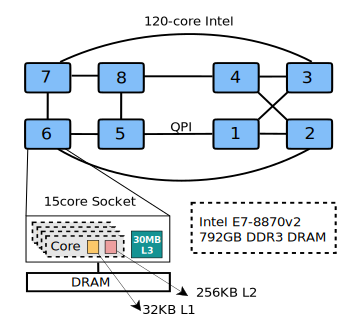
\includegraphics[scale=0.8]{fig/xeon}
\end{center}
\end{frame}

\begin{frame}{Benchmark - BigDataBench}
\begin{center}
\includegraphics[scale=0.5]{fig/benchmark}
\end{center}
\end{frame}

\begin{frame}{Spark Scale-up Server Scalability Problems}
\pgfdeclareimage[width=\paperwidth]{2_problem_1}{.//slides/2_problem_1}
\begin{textblock}{1}(0,0)
\pgfuseimage<+->{2_problem_1}
\end{textblock} 
\end{frame}

\begin{frame}{Spark Scale-up Server Scalability Problems}
\pgfdeclareimage[width=\paperwidth]{2_problem_2}{.//slides/2_problem_2}
\begin{textblock}{1}(0,0)
\pgfuseimage<+->{2_problem_2}
\end{textblock} 
\end{frame}

\begin{frame}{Spark Scale-up Server Scalability Problems}
\pgfdeclareimage[width=\paperwidth]{2_problem_3}{.//slides/2_problem_3}
\begin{textblock}{1}(0,0)
\pgfuseimage<+->{2_problem_3}
\end{textblock} 
\end{frame}

\begin{frame}{The General Scalability Problems}
    \begin{itemize}[<+-| alert@+>]
    \item Garbage Collection(GC) overheads.
    \item Locality of memory accesses on Non-Uniform Memory Access(NUMA)
    architecture.
    \end{itemize}
\end{frame}

\begin{frame}{Effect of Garbage Collection }
\pgfdeclareimage[width=\paperwidth]{3_GC_1}{.//slides/3_GC_1}
\begin{textblock}{1}(0,0)
\pgfuseimage<+->{3_GC_1}
\end{textblock} 
\end{frame}

\begin{frame}{Effect of Garbage Collection}
\pgfdeclareimage[width=\paperwidth]{3_GC_2}{.//slides/3_GC_2}
\begin{textblock}{1}(0,0)
\pgfuseimage<+->{3_GC_2}
\end{textblock} 
\end{frame}

\begin{frame}{Benefit of JVM Partitioning}
\begin{center}
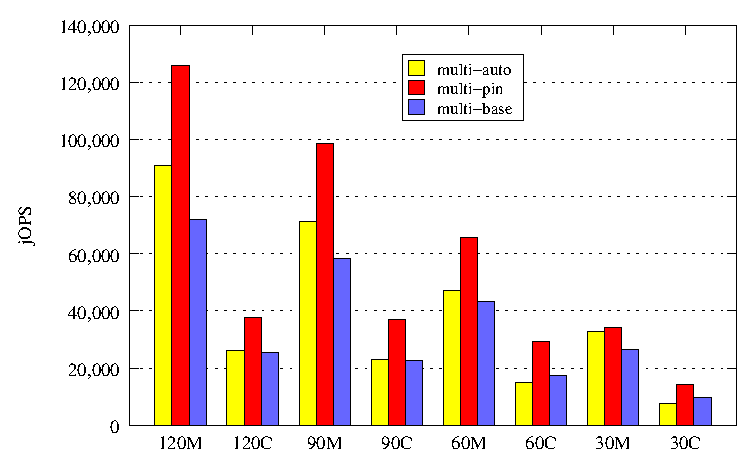
\includegraphics[scale=0.9]{graph/SPECjbb2013}
\end{center}
\end{frame}

\begin{frame}{Proposed Solution - Docker container-based partitioning}
\pgfdeclareimage[width=\paperwidth]{4_Docker}{.//slides/4_Docker}
\begin{textblock}{1}(0,0)
\pgfuseimage<+->{4_Docker}
\end{textblock} 
\end{frame}

\begin{frame}{Benefit of Container-based Partitioning - WC}
\pgfdeclareimage[width=\paperwidth]{5_benefit_wc}{.//slides/5_benefit_wc}
\begin{textblock}{1}(0,0)
\pgfuseimage<+->{5_benefit_wc}
\end{textblock} 
\end{frame}

\begin{frame}{Benefit of Container-based Partitioning - WC}
\pgfdeclareimage[width=\paperwidth]{5_benefit_wc_15}{.//slides/5_benefit_wc_15}
\begin{textblock}{1}(0,0)
\pgfuseimage<+->{5_benefit_wc_15}
\end{textblock} 
\end{frame}

\begin{frame}{Benefit of Container-based Partitioning - WC}
\pgfdeclareimage[width=\paperwidth]{5_benefit_wc_30}{.//slides/5_benefit_wc_30}
\begin{textblock}{1}(0,0)
\pgfuseimage<+->{5_benefit_wc_30}
\end{textblock} 
\end{frame}

\begin{frame}{Benefit of Container-based Partitioning - K-means}
\pgfdeclareimage[width=\paperwidth]{6_benefit_k}{.//slides/6_benefit_k}
\begin{textblock}{1}(0,0)
\pgfuseimage<+->{6_benefit_k}
\end{textblock} 
\end{frame}

\begin{frame}{Benefit of Container-based Partitioning - K-means}
\pgfdeclareimage[width=\paperwidth]{6_benefit_k_15}{.//slides/6_benefit_k_15}
\begin{textblock}{1}(0,0)
\pgfuseimage<+->{6_benefit_k_15}
\end{textblock} 
\end{frame}

\begin{frame}{Straggler Tasks Problem}
\begin{center}
\includegraphics[scale=0.3]{fig/straggler}
\end{center}
Source: http://slideplayer.com/slide/3315804/
\end{frame}

\begin{frame}{Benefit of Container-based Partitioning - K-means}
\pgfdeclareimage[width=\paperwidth]{6_benefit_k_30}{.//slides/6_benefit_k_30}
\begin{textblock}{1}(0,0)
\pgfuseimage<+->{6_benefit_k_30}
\end{textblock} 
\end{frame}

\begin{frame}{Proposed architecture - Design Consideration}
    \begin{itemize}
    \item Finding best-fit CPU counts.
    \item Solving the straggler tasks(i.e, tasks take significantly longer than
    expected to complete) problem.
    \item Improving the NUMA locality.
    \item Avoiding operating systems noise.
    \end{itemize}
\end{frame}

\begin{frame}{Proof-of-concept architecture}
\begin{center}
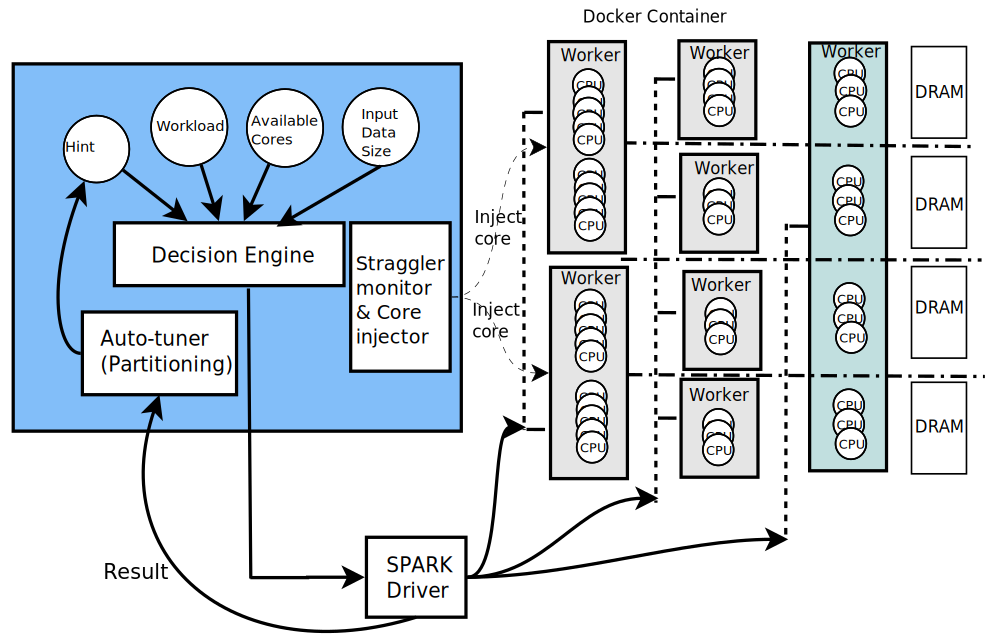
\includegraphics[scale=0.4]{fig/jaildocker}
\end{center}
\end{frame}

\begin{frame}{Future Directions}
\begin{itemize}
\item \textbf{Implementing the proof-of-concept architecture.} 
%This paper shows manually partitioning method, so we will implement the
%Docker-container-based partitioning method.
\item \textbf{Solving the straggler tasks problem.} 
%straggler tasks significantly extend job completion times.
%To mitigate this problem, we may use dynamic resource allocation solution in
%Docker to maximized CPU utilization.
\end{itemize}
\end{frame}

\begin{frame}{Q n A}
\pgfdeclareimage[width=\paperwidth]{10_qna}{.//slides/10_qna}
\begin{textblock}{1}(0,0)
\pgfuseimage<+->{10_qna}
\end{textblock}
\end{frame}


\end{document}
